\documentclass[14pt]{extbook}
\usepackage{multicol, enumerate, enumitem, hyperref, color, soul, setspace, parskip, fancyhdr} %General Packages
\usepackage{amssymb, amsthm, amsmath, bbm, latexsym, units, mathtools} %Math Packages
\everymath{\displaystyle} %All math in Display Style
% Packages with additional options
\usepackage[headsep=0.5cm,headheight=12pt, left=1 in,right= 1 in,top= 1 in,bottom= 1 in]{geometry}
\usepackage[usenames,dvipsnames]{xcolor}
\usepackage{dashrule}  % Package to use the command below to create lines between items
\newcommand{\litem}[1]{\item#1\hspace*{-1cm}\rule{\textwidth}{0.4pt}}
\pagestyle{fancy}
\lhead{Makeup Progress Quiz 3}
\chead{}
\rhead{Version A}
\lfoot{4315-3397}
\cfoot{}
\rfoot{Fall 2020}
\begin{document}

\begin{enumerate}
\litem{
Determine the vertical asymptotes and holes in the rational function below.\[ f(x) = \frac{16x^{3} -49 x + 30}{8x^{2} +2 x -15} \]\begin{enumerate}[label=\Alph*.]
\item \( \text{Vertical Asymptotes of } x = -1.5 \text{ and } x = 1.25 \text{ with no holes.} \)
\item \( \text{Vertical Asymptotes of } x = -1.5 \text{ and } x = 0.75 \text{ with a hole at } x = 1.25 \)
\item \( \text{Holes at } x = -1.5 \text{ and } x = 1.25 \text{ with no vertical asymptotes.} \)
\item \( \text{Vertical Asymptote of } x = 2.0 \text{ and hole at } x = 1.25 \)
\item \( \text{Vertical Asymptote of } x = -1.5 \text{ and hole at } x = 1.25 \)

\end{enumerate} }
\litem{
Determine the vertical asymptotes and holes in the rational function below.\[ f(x) = \frac{12x^{3} -19 x^{2} -45 x -18}{6x^{2} -11 x -10} \]\begin{enumerate}[label=\Alph*.]
\item \( \text{Vertical Asymptotes of } x = 2.5 \text{ and } x = -0.667 \text{ with no holes.} \)
\item \( \text{Vertical Asymptote of } x = 2.5 \text{ and hole at } x = -0.667 \)
\item \( \text{Vertical Asymptote of } x = 2.0 \text{ and hole at } x = -0.667 \)
\item \( \text{Holes at } x = 2.5 \text{ and } x = -0.667 \text{ with no vertical asymptotes.} \)
\item \( \text{Vertical Asymptotes of } x = 2.5 \text{ and } x = -0.75 \text{ with a hole at } x = -0.667 \)

\end{enumerate} }
\litem{
Determine the horizontal and/or oblique asymptotes in the rational function below.\[ f(x) = \frac{3x^{2} -20 x + 25}{18x^{3} -51 x^{2} +5 x + 50} \]\begin{enumerate}[label=\Alph*.]
\item \( \text{Oblique Asymptote of } y = 6x + 23. \)
\item \( \text{Horizontal Asymptote of } y = 0.167  \)
\item \( \text{Horizontal Asymptote at } y = 5.000 \)
\item \( \text{Horizontal Asymptote of } y = 0 \)
\item \( \text{Horizontal Asymptote of } y = 0.167 \text{ and Oblique Asymptote of } y = 6x + 23 \)

\end{enumerate} }
\litem{
Which of the following functions \textit{could} be the graph below?
\begin{center}
    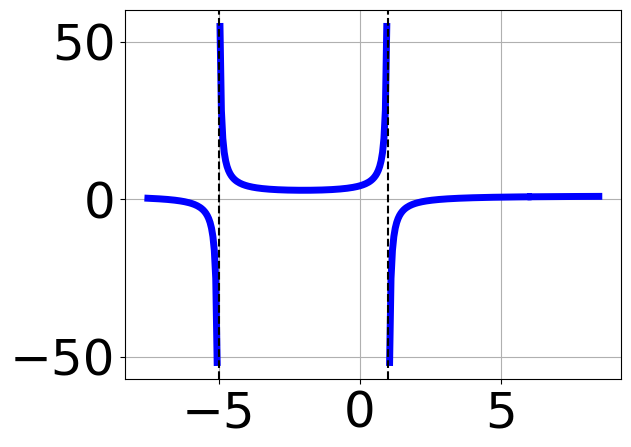
\includegraphics[width=0.5\textwidth]{../Figures/identifyGraphOfRationalFunctionA.png}
\end{center}
\begin{enumerate}[label=\Alph*.]
\item \( f(x)=\frac{x^{3} +5 x^{2} -17 x -21}{x^{3} -2 x^{2} -29 x + 30} \)
\item \( f(x)=\frac{x^{3} +2 x^{2} -45 x -126}{x^{3} +2 x^{2} -29 x -30} \)
\item \( f(x)=\frac{x^{3} +2 x^{2} -45 x -126}{x^{3} +2 x^{2} -29 x -30} \)
\item \( f(x)=\frac{x^{3} -2 x^{2} -45 x + 126}{x^{3} -2 x^{2} -29 x + 30} \)
\item \( \text{None of the above are possible equations for the graph.} \)

\end{enumerate} }
\litem{
Determine the horizontal and/or oblique asymptotes in the rational function below.\[ f(x) = \frac{12x^{3} -71 x^{2} +130 x -75}{3x^{2} -17 x + 20} \]\begin{enumerate}[label=\Alph*.]
\item \( \text{Oblique Asymptote of } y = 4x -1. \)
\item \( \text{Horizontal Asymptote of } y = 4.0 \text{ and Oblique Asymptote of } y = 4x -1 \)
\item \( \text{Horizontal Asymptote at } y = 4.0 \)
\item \( \text{Horizontal Asymptote of } y = 4.0  \)
\item \( \text{Horizontal Asymptote of } y = 4.0 \text{ and Oblique Asymptote of } y = 4x -1 \)

\end{enumerate} }
\litem{
Determine the horizontal and/or oblique asymptotes in the rational function below.\[ f(x) = \frac{2x^{2} +13 x + 20}{8x^{3} +6 x^{2} -65 x -75} \]\begin{enumerate}[label=\Alph*.]
\item \( \text{Oblique Asymptote of } y = 4x -23. \)
\item \( \text{Horizontal Asymptote of } y = 0 \)
\item \( \text{Horizontal Asymptote at } y = -4.000 \)
\item \( \text{Horizontal Asymptote of } y = 0.250 \text{ and Oblique Asymptote of } y = 4x -23 \)
\item \( \text{Horizontal Asymptote of } y = 0.250  \)

\end{enumerate} }
\litem{
Determine the vertical asymptotes and holes in the rational function below.\[ f(x) = \frac{4x^{3} -12 x^{2} -31 x + 60}{6x^{2} -x -12} \]\begin{enumerate}[label=\Alph*.]
\item \( \text{Vertical Asymptotes of } x = -1.333 \text{ and } x = -2.5 \text{ with a hole at } x = 1.5 \)
\item \( \text{Holes at } x = -1.333 \text{ and } x = 1.5 \text{ with no vertical asymptotes.} \)
\item \( \text{Vertical Asymptote of } x = 0.667 \text{ and hole at } x = 1.5 \)
\item \( \text{Vertical Asymptotes of } x = -1.333 \text{ and } x = 1.5 \text{ with no holes.} \)
\item \( \text{Vertical Asymptote of } x = -1.333 \text{ and hole at } x = 1.5 \)

\end{enumerate} }
\litem{
Which of the following functions \textit{could} be the graph below?
\begin{center}
    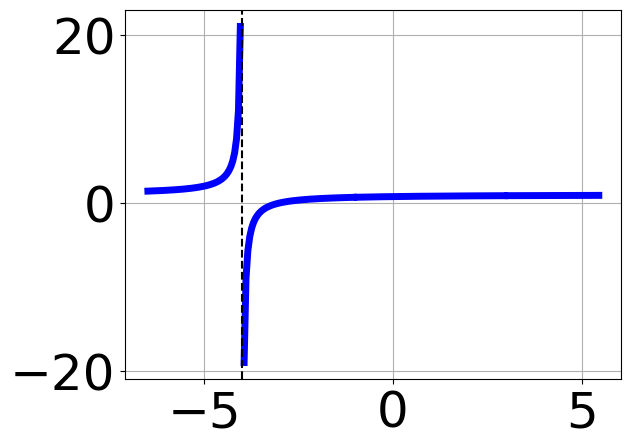
\includegraphics[width=0.5\textwidth]{../Figures/identifyGraphOfRationalFunctionCopyA.png}
\end{center}
\begin{enumerate}[label=\Alph*.]
\item \( f(x)=\frac{x^{3} -1 x^{2} -9 x + 9}{x^{3} -2 x^{2} -11 x + 12} \)
\item \( f(x)=\frac{x^{3} + x^{2} -9 x -9}{x^{3} +2 x^{2} -11 x -12} \)
\item \( f(x)=\frac{x^{3} +13 x^{2} +51 x + 63}{x^{3} +2 x^{2} -11 x -12} \)
\item \( f(x)=\frac{x^{3} -1 x^{2} -9 x + 9}{x^{3} -2 x^{2} -11 x + 12} \)
\item \( \text{None of the above are possible equations for the graph.} \)

\end{enumerate} }
\litem{
Determine the horizontal and/or oblique asymptotes in the rational function below.\[ f(x) = \frac{16x^{3} -32 x^{2} -113 x -60}{4x^{2} -17 x -15} \]\begin{enumerate}[label=\Alph*.]
\item \( \text{Horizontal Asymptote of } y = 5.0 \text{ and Oblique Asymptote of } y = 4x + 9 \)
\item \( \text{Horizontal Asymptote of } y = 4.0  \)
\item \( \text{Horizontal Asymptote at } y = 5.0 \)
\item \( \text{Horizontal Asymptote of } y = 4.0 \text{ and Oblique Asymptote of } y = 4x + 9 \)
\item \( \text{Oblique Asymptote of } y = 4x + 9. \)

\end{enumerate} }
\litem{
Determine the vertical asymptotes and holes in the rational function below.\[ f(x) = \frac{6x^{3} -35 x^{2} +66 x -40}{8x^{2} -30 x + 25} \]\begin{enumerate}[label=\Alph*.]
\item \( \text{Holes at } x = 1.25 \text{ and } x = 2.5 \text{ with no vertical asymptotes.} \)
\item \( \text{Vertical Asymptote of } x = 0.75 \text{ and hole at } x = 2.5 \)
\item \( \text{Vertical Asymptote of } x = 1.25 \text{ and hole at } x = 2.5 \)
\item \( \text{Vertical Asymptotes of } x = 1.25 \text{ and } x = 2.5 \text{ with no holes.} \)
\item \( \text{Vertical Asymptotes of } x = 1.25 \text{ and } x = 1.333 \text{ with a hole at } x = 2.5 \)

\end{enumerate} }
\end{enumerate}

\end{document}